\subsection{ViewModel}
\label{chap:viewmodel_design}
The \emph{view model} is responsible for providing the necessary data and functionality to the \emph{view}, resulting in a clear separation between the \emph{view} and the \emph{model}.
The system consists of three \emph{view models}, namely \texttt{HrViewModel}, responsible for managing business logics related to heart rate and activity data, \texttt{ExerciseViewModel}, which manages business logics for exercise related data, and lastly \texttt{UserViewModel}, responsible for managing business logics related to user.

\subsubsection{HrViewModel}
\label{chap:hrviewmodel_design}
The \texttt{HrViewModel} is responsible for managing business logics related to the heart rate data and activity within the system.
This \emph{view model} facilitates the communication between the \texttt{HomeFragment} and the business logics related to the heart rate data and activity, for instance, \texttt{ConnectionService} and \texttt{ActivityService}.
Additionally, it includes heart rate LiveData\footnote{\emph{LiveData} is an observable data holder class. LiveData follows the observable pattern and allows other components to observe changes in the data. URL: \url{https://developer.android.com/topic/libraries/architecture/livedata}} and activity LiveData, enabling the fragment to observe these data and receive updates whenever changes occur. This allows fragment to react accordingly and adjust the user interface correspondingly.
Furthermore, the \texttt{HrViewModel} interacts with the repositories to perform necessary operations on heart rate data.
Sequence diagrams are created to visually represent the sequence of operations executed in \texttt{HrViewModel}.

\begin{figure}[H]
    \centering
    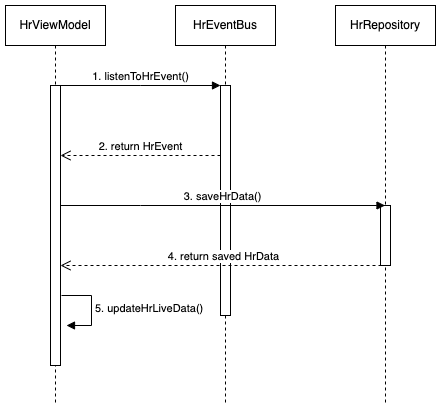
\includegraphics[width=0.7\textwidth]{diagrams/hrviewmodel-hr.drawio.png}
    \caption{HrViewModel heart rate data flow sequence diagram}
    \label{fig:hrviewmodel_hrdata}
\end{figure}

To provide the \texttt{HomeFragment} with the actual heart rate data, the following sequence of operations visualized in \autoref{fig:hrviewmodel_hrdata} is executed:
\begin{enumerate}
    \item The \texttt{HrViewModel} actively listens to events published by the \texttt{ConnectionService} to \texttt{HrEventBus}.
    \item Event containing heart rate data is retrieved.
    \item Heart rate from the event is extracted and sent to \texttt{HrRepository} to be persisted to the database.
    \item Once the heart rate data has successfully been saved, it will be returned to \texttt{HrViewModel}.
    \item \texttt{HrViewModel} updates the heart rate LiveData.
\end{enumerate}

The following sequence of operations is visualized in \autoref{fig:hrviewmodel_activitydata} and is executed to provide the \texttt{HomeFragment} with up-to-date activity data.
\begin{enumerate}
    \item The \texttt{HrViewModel} actively listens to events published in \texttt{ActivityEventBus}.
    \item Event containing activity data is retrieved.
    \item \texttt{HrViewModel} updates the activity LiveData with the retrieved activity data.
\end{enumerate}

\begin{figure}[H]
    \centering
    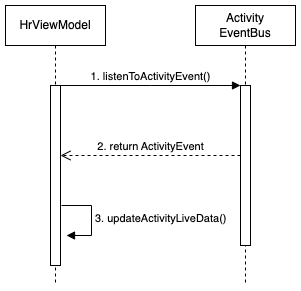
\includegraphics[width=0.5\textwidth]{diagrams/hrviewmodel-activity.drawio.png}
    \caption{HrViewModel activity data flow sequence diagram}
    \label{fig:hrviewmodel_activitydata}
\end{figure}

\subsubsection{ExerciseViewModel}
\label{chap:exerciseviewmodel_design}
The \texttt{ExerciseViewModel} is responsible for managing business logics related to exercise within the application.
It supports the communication between the \texttt{ExerciseFragment} and the business logics related to exercise such as the \texttt{ExerciseService}.
The \texttt{ExerciseViewModel} also manages the current exercise LiveData, which holds the current exercise data and is observed by the \texttt{ExerciseFragment} for real-time updates. 
Additionally, the ExerciseViewModel interacts with other components, for instance, the repositories to perform necessary operations to manage data.

\begin{figure}[H]
    \centering
    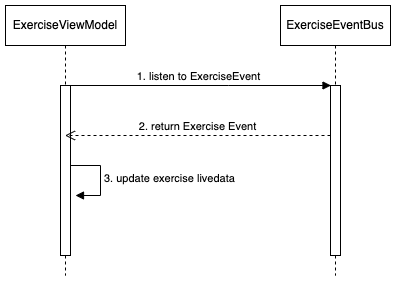
\includegraphics[width=0.7\textwidth]{diagrams/exercise-view-model-seq.drawio.png}
    \caption{ExerciseViewModel exercise data flow sequence diagram}
    \label{fig:exerciseviewmodel_exercisedata}
\end{figure}
To support the \texttt{ExerciseFragment} with the actual exercise data, the following sequence of operations is illustrated in \autoref{fig:exerciseviewmodel_exercisedata}:
\begin{enumerate}
    \item The \texttt{ExerciseViewModel} actively listens to events published in \texttt{ExerciseEventBus}.
    \item Event containing exercise data is retrieved.
    \item The \texttt{ExerciseViewModel} updates the exercise LiveData with the retrieved exercise data.
\end{enumerate}

\subsubsection{UserViewModel}
\label{chap:userviewmodel_design}
The \texttt{UserViewModel} is responsible for managing business logics related to user within the application.
It provides the necessary functionalities and data access methods to manage and manipulate user-related information. 
The \texttt{UserViewModel} handles tasks such as adding a new user, updating user data, switching active user, and deleting a user, including all of their data.
To support those functionalities, the \texttt{UserViewModel} maintains close connection to the repository to retrieve user data, update user information, and perform other user-related operations. 
Additionally, to ensure that the \texttt{UserFragment} reflects the most up-to-date user information, the \texttt{UserViewModel} exposes active user LiveData and user list LiveData to the \texttt{UserFragment}.
The active user LiveData contains information regarding the current active user, while the user list LiveData provides a list of available users in the database.

System sequences can now be defined as a result of analyzing the following user story:
\begin{quotation}
    \enquote{As a user of the application who is concerned about data privacy, I want to be able to manage and control my user profile easily.}
\end{quotation}
Sequence diagrams have been created to provide a better overview of the functionalities offered by the \texttt{UserViewModel}. These diagrams illustrate the sequence of interactions and method calls between the \texttt{UserViewModel} , the repository, and other relevant components.

The following sequence of operations displayed in \autoref{fig:userviewmodel_upsertuser} is executed to support the functionality to add and update new user.
\begin{enumerate}
    \item The \texttt{UserViewModel} receives a request to update or insert user.
    \item The request is forwarded to \texttt{UserRepository} to be persisted in the database. Room database automatically searches for existing user in the database, if no user is found, it creates a new user, otherwise it updates the user.
    \item Once the user is successfully saved within the database, it is returned.
    \item The user list live data is updated with the saved user.
    \item The saved user is set as active.
    \item The \texttt{UserViewModel} updates the active user live data.
\end{enumerate}

\begin{figure}[H]
    \centering
    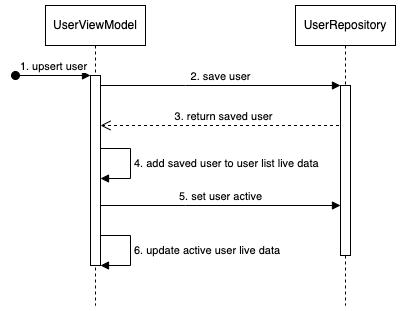
\includegraphics[width=0.8\textwidth]{diagrams/upsert-user-vm.drawio.png}
    \caption{UserViewModel add or update user sequence diagram}
    \label{fig:userviewmodel_upsertuser}
\end{figure}

The functionality to delete user is supported through the following sequence of operations and it is visualized in \autoref{fig:userviewmodel_deleteuser}

\begin{enumerate}
    \item The \texttt{UserViewModel} receives a request to delete user.
    \item \texttt{ServiceRunningChecker} validates if there are any running services
    \item Validation result is returned
    \item if there are no service running, \texttt{UserRepository} deletes the user.
    \item Once the user is successfully deleted, the last created user is marked as active.
    \item The \texttt{UserViewModel} updates the active user live data.
\end{enumerate}

Alternate sequence
\begin{enumerate}[start=4]
    \item If the validation fails, error will be thrown and \texttt{UserFragment} notifies the user.
\end{enumerate}

\begin{figure}[H]
    \centering
    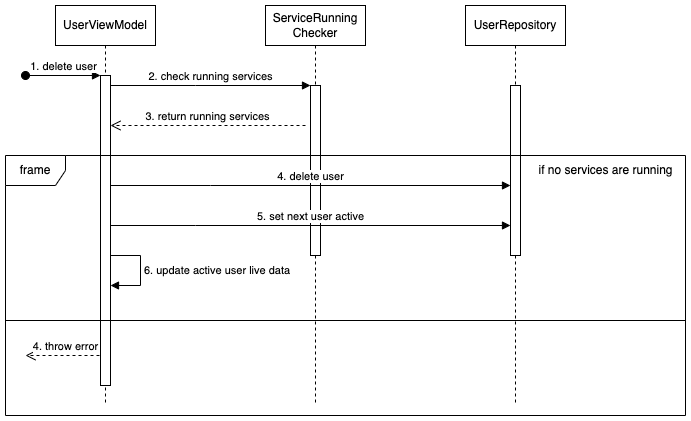
\includegraphics[width=1\textwidth]{diagrams/delete-user-vm.drawio.png}
    \caption{UserViewModel delete user sequence diagram}
    \label{fig:userviewmodel_deleteuser}
\end{figure}

